\documentclass{beamer}
\usetheme{Madrid}
\usecolortheme{default}

\usepackage[utf8]{inputenc}
\usepackage[T1]{fontenc}
\usepackage[magyar]{babel}
\usepackage{amsmath, amssymb}
\usepackage{tikz}
\usepackage{tcolorbox}

\title{Ismétlés nélküli permutáció}
\author{Varga Dávid}
\institute{Matematika}
\date{}

%%% Megjelenítéshez automatikusan kiegészített csomagok %%%
\usepackage{amsfonts}
\usepackage{xcolor}
\usepackage{pgfplots}
\pgfplotsset{compat=1.18}
\usepackage{graphicx}
\usepackage{enumitem}
\usepackage{booktabs}
\usepackage{float}
\usepackage{caption}
\usepackage{microtype}

\usepackage{hyperref}

\begin{document}

\begin{frame}
    \titlepage
\end{frame}

\begin{frame}{1. A lényeg}
    \begin{block}{Definíció}
        Képzeld el, hogy van pár teljesen különböző dolgod, és egyszerűen csak sorba akarod rendezni őket. Az \textbf{ismétlés nélküli permutáció} nem más, mint annak a kiszámítása, hogy hányféleképpen állíthatod sorba ezeket a dolgokat úgy, hogy mindegyiket pontosan egyszer használod fel.
    \end{block}

    \vspace{0.5cm}
    \begin{center}
        \emph{Hogyan számolhatjuk ki ezeket a lehetőségeket? Nézzünk egy példát!}
    \end{center}
\end{frame}

\begin{frame}{2. Hogyan is működik?}
    \small
    Gondolj arra, hogy van három barát: Anna, Balázs és Csaba, és be akarnak ülni a moziba három egymás melletti székre. Hányféleképpen ülhetnek le?
    
    \begin{itemize}
        \item \textbf{1. szék:} Bárki leülhet $\rightarrow$ \textbf{3} lehetőség.
        \item \textbf{2. szék:} A maradék kettő közül valaki $\rightarrow$ \textbf{2} lehetőség.
        \item \textbf{3. szék:} Aki maradt $\rightarrow$ \textbf{1} lehetőség.
    \end{itemize}

    \vspace{0.3cm}
    \begin{center}
        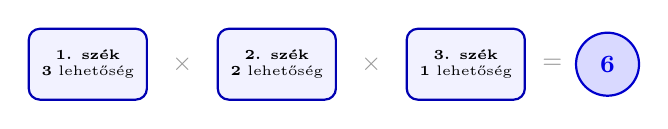
\begin{tikzpicture}[
            szek/.style={draw=blue!70!black, fill=blue!5, thick, rounded corners=4pt, align=center, minimum width=1.5cm, minimum height=0.9cm, font=\tiny},
            muvelet/.style={font=\small\bfseries, text=gray!80},
            eredmeny/.style={draw=blue!80!black, fill=blue!15, circle, thick, minimum size=0.8cm, font=\small\bfseries, text=blue!90!black}
        ]
            \node[szek] (c1) at (0,0) {\textbf{1. szék}\\\textbf{3} lehetőség};
            \node[muvelet] at (1.2,0) {$\times$};
            \node[szek] (c2) at (2.4,0) {\textbf{2. szék}\\\textbf{2} lehetőség};
            \node[muvelet] at (3.6,0) {$\times$};
            \node[szek] (c3) at (4.8,0) {\textbf{3. szék}\\\textbf{1} lehetőség};
            \node[muvelet] at (5.9,0) {$=$};
            \node[eredmeny] at (6.6,0) {6};
        \end{tikzpicture}
    \end{center}
    
    \vspace{0.2cm}
    \textbf{Miért szorzunk?} Mert a döntések egymásba ágyazódnak (fa-diagram elv): minden esethez a többinél újabb események tartoznak. Végeredmény: $3 \cdot 2 \cdot 1 = 6$.
\end{frame}

\begin{frame}{3. Általános képlet és határesetek}
    \begin{block}{Általános képlet ($P_n$)}
        Ha $n$ darab különböző elemünk van, az összes lehetséges sorrendjének a száma:
        $$P_n = n! = n \cdot (n - 1) \cdot (n - 2) \cdot \dots \cdot 1$$
        Ahol a felkiáltójel neve: \textbf{faktoriális}.
    \end{block}

    \vspace{0.3cm}
    \textbf{Fontos tudnivalók:}
    \begin{itemize}
        \item \textbf{Feltétel:} Csak akkor használható, ha az elemek \textbf{különböznek} egymástól (nincs duplikáció).
        \item \textbf{A nulla faktoriális:} $0! = 1$. (Ha nulla dolgot kell sorbaraknod, azt pontosan 1-féleképpen teheted meg).
    \end{itemize}
\end{frame}

\begin{frame}{4. Dolgozat gyorsteszt}
    \begin{alertblock}{A 3 pontos ellenőrzés}
        Amikor a dolgozatban meglátsz egy feladatot, futtasd le ezt a 3 kérdést. Ha mindháromra \textbf{IGEN} a válasz, a képleted az $n!$:
    \end{alertblock}

    \begin{enumerate}
        \item \textbf{Ugyanannyi a hely, mint az elem?} \par (Mindenkit leültetünk? Nem marad ki senki?)
        \item \textbf{Számít a sorrend?} \par (Anna-Balázs $\neq$ Balázs-Anna?)
        \item \textbf{Minden elem különbözik?} \par (Nincsenek egyforma tárgyak/klónok?)
    \end{enumerate}
\end{frame}

\begin{frame}{5. Tipikus feladatok: Alap és Ragasztós trükk}
    \small
    \textbf{1. Alapfeladat (Mozis sor):} \\
    \emph{5 fős társaság moziba megy, 5 székre ülnek.}
    \begin{itemize}
        \item Megoldás: $5! = 5 \cdot 4 \cdot 3 \cdot 2 \cdot 1 = \mathbf{120}$ lehetőség.
    \end{itemize}
\end{frame}

    \vspace{0.3cm}
    \textbf{2. A "ragasztós" trükk (Összetartozó elemek):} \\
    \emph{5 ember ül le, de Béla és Cili egymás mellett akar ülni.}
    \begin{itemize}
        \item \textbf{1. lépés:} Bélát és Cilit összeragasztjuk $\rightarrow$ 4 "csomag" van ($4!$).
        \item \textbf{2. lépés:} A pároson belül helycsere is van ($2!$).
        \item Megoldás: $4! \cdot 2! = 24 \cdot 2 = \mathbf{48}$ lehetőség.
    \end{itemize}
\end{frame}

\begin{frame}{5. Tipikus feladatok: Kizárás és Korlátozás}
    \small
    \textbf{3. Kizárási feladat (Egymás mellett nem állók):} \\
    \emph{5 ember ül le, de Anna és Béla NEM ülhet egymás mellett.}
    \begin{itemize}
        \item Összes eset ($5! = 120$) $-$ Tiltott esetek ($4! \cdot 2! = 48$) $= \mathbf{72}$.
    \end{itemize}

    \vspace{0.3cm}
    \textbf{4. Korlátozó feltétel (Fixált helyek / Nullás feladat):} \\
    \emph{0, 1, 2, 3, 4 számjegyekből hány 5-jegyű szám képezhető?}
    \begin{itemize}
        \item \textbf{1. hely:} A nulla nem állhat elöl $\rightarrow$ 4 lehetőség.
        \item \textbf{Maradék helyek:} 4 elem marad a 4 helyre $\rightarrow$ $4!$ lehetőség.
        \item Megoldás: $4 \cdot 4! = 4 \cdot 24 = \mathbf{96}$ darab szám.
    \end{itemize}
\end{frame}

\begin{frame}{5. Tipikus feladatok: Körmutáció és Paritás}
    \small
    \textbf{5. Ciklikus / Körmutáció:} \\
    \emph{5 ember kerek asztal körül (forgatással megegyezők azonosak).}
    \begin{itemize}
        \item Egy embert rögzítünk, a többit permutáljuk: $(n-1)! = 4! = \mathbf{24}$.
    \end{itemize}

    \vspace{0.2cm}
    \textbf{6. Kötött pozíció:} \\
    \emph{6 versenyző, de a leggyorsabb (A) biztosan az 1. helyen végez.}
    \begin{itemize}
        \item 1. hely fix (1), a többi 5 szabad ($5!$): $1 \cdot 5! = \mathbf{120}$.
    \end{itemize}

    \vspace{0.2cm}
    \textbf{7. Váltakozó elrendezés:} \\
    \emph{3 fiú és 3 lány váltakozva ül egy sorban.}
    \begin{itemize}
        \item Mintázat (2) $\times$ Fiúk ($3!$) $\times$ Lányok ($3!$): $2 \cdot 6 \cdot 6 = \mathbf{72}$.
    \end{itemize}
\end{frame}

\begin{frame}
    \centering
    \Huge Köszönöm a figyelmet!
\end{frame}

\end{document}